% ==============================================================================
% PAGE 15: CHAPTER-3 METHODOLOGY - 1) PARABOLIC DISH (Numbered Page 7)
% ==============================================================================
\begin{center}
  {\fontsize{15}{18}\selectfont \bfseries \textcolor{red!80!black}{\underline{CHAPTER-3}}}\\[2mm]
  {\fontsize{16}{20}\selectfont \bfseries \textcolor{red!80!black}{\underline{METHODOLOGY}}}\\[4mm]
\end{center}

\subsection*{3.1 DESING PARAMETER AND SELECTION OF COMPONANTS}
\subsubsection*{1) PARABOLIC DISH}

\begin{center}
  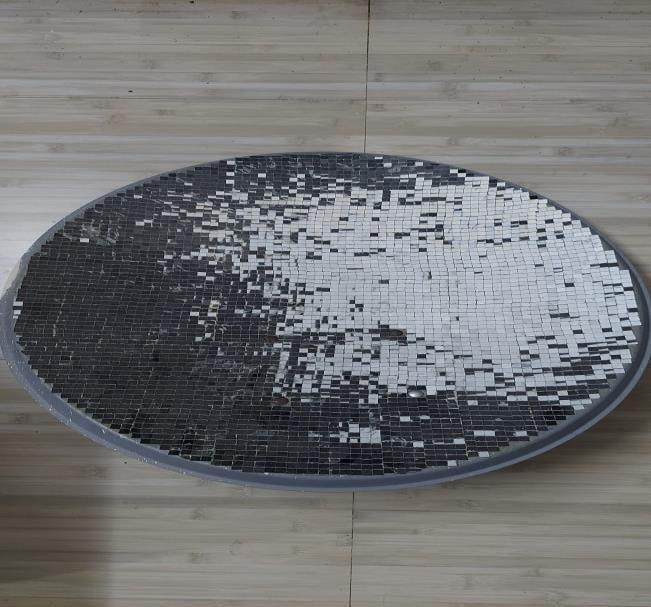
\includegraphics[width=68mm]{figures/fig1_parabolic_dish.jpg}
\end{center}

\vspace{2mm}
\noindent
\begin{spacing}{1.15}
{\fontsize{9.8}{13.5}\selectfont
The image shows the fabricated parabolic solar concentrator developed for this project, which is designed to focus sunlight onto a single focal point for efficient heat generation. The concentrator surface is constructed using multiple small square mirror pieces carefully arranged on a curved parabolic base to achieve the desired reflective geometry. Each mirror segment reflects incoming solar radiation toward the focal point, where a receiver tube or container is placed to absorb concentrated heat energy. This design allows the system to attain high temperatures suitable for water heating and steam generation, utilizing clean and renewable solar energy.\\[2.5mm]
The use of mirror tiles instead of a single reflective sheet significantly reduces fabrication costs while maintaining high reflectivity and durability. The circular structure provides better light focusing and structural stability. The concentrator, with a 60~cm diameter and 40~cm focal length, is integrated with a real-time automated solar tracking system to maintain optimal alignment with the sun throughout the day. This practical and cost-effective design demonstrates the potential of locally fabricated solar concentrators for sustainable thermal energy applications in domestic and industrial sectors. A parabolic concentrator is a reflective device that focuses incoming solar radiation onto a focal point or line. The design is based on the geometric properties of a parabola, where all rays parallel to the principal axis are reflected through a single focal point. In this project, a cylindrical parabolic concentrator is used to concentrate sunlight onto a receiver tube located at the focal point to achieve efficient heating and steam generation.
}
\end{spacing}
\clearpage
